%We computed the SDC probabilities of the AN codes with \(|A| \leq 16\), whereby the 
%We now show how we computed the SDC probabilities of the AN codes with \(|A| \leq 16\). For the following, we reuse the definitions from Section~\ref{sec:ANCoding}.

 % Runtime AN-Coding exact, AN-Coding qMC M {Runtime, max.rel.err}, Hamming {Runtime, max.rel.err}
% M = 0.01*2^k
\begin{table}%[!hb]
	\centering
	\sisetup{
		round-mode=places,
		round-precision=0
	}
	\renewcommand{\arraystretch}{1.2}
	\begin{tabular}{@{}lrrrrrrrr@{}}
		\toprule
		& \multicolumn{3}{c}{exact} & \multicolumn{2}{c}{$\sigma_{\text{grid,1D},4\cdot\mathrm{GPU}}$} & 
		\\[-\aboverulesep]
		\arrayrulecolor[gray]{0.5}\cmidrule(lr){2-4}\cmidrule(lr){5-6}\arrayrulecolor{black}
		$k$ & $t_{\mathrm{CPU}}$ & $t_{1\cdot\mathrm{GPU}}$ & $t_{4\cdot\mathrm{GPU}}$ & $t_M$ & $\Delta_M$ & $M$\\
		\midrule
		8  & \SI{6.786}{\milli\second{}}   & \SI{0.658}{\milli\second{}}   & \SI{3.022}{\milli\second{}}  & \SI{5.856}{\milli\second{}}   & \num[round-precision=4]{0.02321} & 101\\
16 & \SI{375.533}{\milli\second{}} & \SI{129.728}{\milli\second{}} & \SI{40.707}{\milli\second{}} & \SI{10.516}{\milli\second{}}  & \num[round-precision=4]{0.00305} & 1001\\
24 & \SI{382.133}{\minute{}}       & \SI{99.485}{\minute{}}        & \SI{27.019}{\minute{}}       & \SI{353.865}{\milli\second{}} & \num[round-precision=4]{0.00527} & 1001\\
32 & --                            & --                            & --                           & \SI{4.889}{\minute{}}         & --                               & 1001\\

		\bottomrule
	\end{tabular}
	\caption{Computing the distance distributions of AN codes for \(A=61\). Average values after 5 runs.
	% TODO[include] on the Bull HPC-Cluster at TU Dresden.
CPU: 2$\times$E5-2680 v3 Haswell 12-core \SI[round-precision=2]{2.50}{GHz}, gcc5.3, OpenMP 4.0. GPU: NVIDIA Tesla K80, CUDA 7.5}
	\label{tab:runtimes}
	\vspace{-3em}
\end{table}

\section{Computing The SDC Probability}
\label{appendix:SDCProbability}

There is plenty of work on evaluating the probability of undetected errors for linear block codes\footnote{For linear codes, the linear combination (\emph{exclusive} OR) of two valid code words is \emph{always} also a valid code word.} and Hamming code in particular~\cite{KAUR19941141,Wolf1982,moon2005error}. For AN codes, this has only been done for 8- and 16-bit data and \(A\)s up to 8 and 16 bits~\cite{DBLP:conf/hase/HoffmannUDSLS14,coredExperiments}. However, this is insufficient for the database domain, because \begin{inparaenum} \item possibly all data bit widths between 1 and 64 bits are to be supported~\cite{willhalm2013vectorizing}, and \item larger \(A\)s may be required for future error models\end{inparaenum}. To overcome that, we developed a practical methodology for determining the probability of SDC for non-systematic, non-linear\footnote{In non-linear codes, the linearity property is not always satisfied.} coding schemes in general and independent of a specific error model~\cite{kolditz2018}. For this, we use the following definitions: A code \(\mathbb{C}\) (EDC/ECC) is defined by the triplet $(n, k, d_\text{min})$, were $n=|\mathbb{C}|$ is the code word width, $k$ is the data width, and $d_\text{min}$ is the minimum Hamming distance between any of the code's valid code words. Further, $b$ denotes the number of flipped bits. For AN coding, the definitions from Section~\ref{sec:ErrorCoding} further apply.
 


%Moreover, we assume no specific probability for the occurrence of any error patterns and only compute conditional likelihoods. We assume this, because, to the best of our knowledge, there is no error model for future hardware technologies, which would provide us with specific probabilities of the number and rate of bit flips per data unit (byte, word, etc.), or probabilities for certain error patterns. If there is one available, we could well integrate it.

\begin{figure}[t]
	\centering
	{
		\graphicspath{{gnuplot/}}
		% GNUPLOT: LaTeX picture with Postscript
\begingroup
  \makeatletter
  \providecommand\color[2][]{%
    \GenericError{(gnuplot) \space\space\space\@spaces}{%
      Package color not loaded in conjunction with
      terminal option `colourtext'%
    }{See the gnuplot documentation for explanation.%
    }{Either use 'blacktext' in gnuplot or load the package
      color.sty in LaTeX.}%
    \renewcommand\color[2][]{}%
  }%
  \providecommand\includegraphics[2][]{%
    \GenericError{(gnuplot) \space\space\space\@spaces}{%
      Package graphicx or graphics not loaded%
    }{See the gnuplot documentation for explanation.%
    }{The gnuplot epslatex terminal needs graphicx.sty or graphics.sty.}%
    \renewcommand\includegraphics[2][]{}%
  }%
  \providecommand\rotatebox[2]{#2}%
  \@ifundefined{ifGPcolor}{%
    \newif\ifGPcolor
    \GPcolortrue
  }{}%
  \@ifundefined{ifGPblacktext}{%
    \newif\ifGPblacktext
    \GPblacktexttrue
  }{}%
  % define a \g@addto@macro without @ in the name:
  \let\gplgaddtomacro\g@addto@macro
  % define empty templates for all commands taking text:
  \gdef\gplbacktext{}%
  \gdef\gplfronttext{}%
  \makeatother
  \ifGPblacktext
    % no textcolor at all
    \def\colorrgb#1{}%
    \def\colorgray#1{}%
  \else
    % gray or color?
    \ifGPcolor
      \def\colorrgb#1{\color[rgb]{#1}}%
      \def\colorgray#1{\color[gray]{#1}}%
      \expandafter\def\csname LTw\endcsname{\color{white}}%
      \expandafter\def\csname LTb\endcsname{\color{black}}%
      \expandafter\def\csname LTa\endcsname{\color{black}}%
      \expandafter\def\csname LT0\endcsname{\color[rgb]{1,0,0}}%
      \expandafter\def\csname LT1\endcsname{\color[rgb]{0,1,0}}%
      \expandafter\def\csname LT2\endcsname{\color[rgb]{0,0,1}}%
      \expandafter\def\csname LT3\endcsname{\color[rgb]{1,0,1}}%
      \expandafter\def\csname LT4\endcsname{\color[rgb]{0,1,1}}%
      \expandafter\def\csname LT5\endcsname{\color[rgb]{1,1,0}}%
      \expandafter\def\csname LT6\endcsname{\color[rgb]{0,0,0}}%
      \expandafter\def\csname LT7\endcsname{\color[rgb]{1,0.3,0}}%
      \expandafter\def\csname LT8\endcsname{\color[rgb]{0.5,0.5,0.5}}%
    \else
      % gray
      \def\colorrgb#1{\color{black}}%
      \def\colorgray#1{\color[gray]{#1}}%
      \expandafter\def\csname LTw\endcsname{\color{white}}%
      \expandafter\def\csname LTb\endcsname{\color{black}}%
      \expandafter\def\csname LTa\endcsname{\color{black}}%
      \expandafter\def\csname LT0\endcsname{\color{black}}%
      \expandafter\def\csname LT1\endcsname{\color{black}}%
      \expandafter\def\csname LT2\endcsname{\color{black}}%
      \expandafter\def\csname LT3\endcsname{\color{black}}%
      \expandafter\def\csname LT4\endcsname{\color{black}}%
      \expandafter\def\csname LT5\endcsname{\color{black}}%
      \expandafter\def\csname LT6\endcsname{\color{black}}%
      \expandafter\def\csname LT7\endcsname{\color{black}}%
      \expandafter\def\csname LT8\endcsname{\color{black}}%
    \fi
  \fi
    \setlength{\unitlength}{0.0500bp}%
    \ifx\gptboxheight\undefined%
      \newlength{\gptboxheight}%
      \newlength{\gptboxwidth}%
      \newsavebox{\gptboxtext}%
    \fi%
    \setlength{\fboxrule}{0.5pt}%
    \setlength{\fboxsep}{1pt}%
\begin{picture}(4740.00,2880.00)%
    \gplgaddtomacro\gplbacktext{%
      \colorrgb{0.27,0.27,0.27}%
      \put(455,558){\makebox(0,0)[r]{\strut{}\scriptsize{$10^{-5}$}}}%
      \colorrgb{0.27,0.27,0.27}%
      \put(455,948){\makebox(0,0)[r]{\strut{}\scriptsize{$10^{-4}$}}}%
      \colorrgb{0.27,0.27,0.27}%
      \put(455,1338){\makebox(0,0)[r]{\strut{}\scriptsize{$10^{-3}$}}}%
      \colorrgb{0.27,0.27,0.27}%
      \put(455,1727){\makebox(0,0)[r]{\strut{}\scriptsize{$10^{-2}$}}}%
      \colorrgb{0.27,0.27,0.27}%
      \put(455,2117){\makebox(0,0)[r]{\strut{}\scriptsize{$10^{-1}$}}}%
      \colorrgb{0.27,0.27,0.27}%
      \put(455,2507){\makebox(0,0)[r]{\strut{}\scriptsize{$10^{0}$}}}%
      \colorrgb{0.27,0.27,0.27}%
      \put(612,317){\makebox(0,0){\strut{}\scriptsize{$10^{1}$}}}%
      \colorrgb{0.27,0.27,0.27}%
      \put(1159,317){\makebox(0,0){\strut{}\scriptsize{$10^{2}$}}}%
      \colorrgb{0.27,0.27,0.27}%
      \put(1706,317){\makebox(0,0){\strut{}\scriptsize{$10^{3}$}}}%
      \colorrgb{0.27,0.27,0.27}%
      \put(2254,317){\makebox(0,0){\strut{}\scriptsize{$10^{4}$}}}%
      \colorrgb{0.27,0.27,0.27}%
      \put(2801,317){\makebox(0,0){\strut{}\scriptsize{$10^{5}$}}}%
      \colorrgb{0.27,0.27,0.27}%
      \put(2958,558){\makebox(0,0)[l]{\strut{}\scriptsize{$10^{-3}$}}}%
      \colorrgb{0.27,0.27,0.27}%
      \put(2958,836){\makebox(0,0)[l]{\strut{}\scriptsize{$10^{-2}$}}}%
      \colorrgb{0.27,0.27,0.27}%
      \put(2958,1115){\makebox(0,0)[l]{\strut{}\scriptsize{$10^{-1}$}}}%
      \colorrgb{0.27,0.27,0.27}%
      \put(2958,1393){\makebox(0,0)[l]{\strut{}\scriptsize{$10^{0}$}}}%
      \colorrgb{0.27,0.27,0.27}%
      \put(2958,1672){\makebox(0,0)[l]{\strut{}\scriptsize{$10^{1}$}}}%
      \colorrgb{0.27,0.27,0.27}%
      \put(2958,1950){\makebox(0,0)[l]{\strut{}\scriptsize{$10^{2}$}}}%
      \colorrgb{0.27,0.27,0.27}%
      \put(2958,2229){\makebox(0,0)[l]{\strut{}\scriptsize{$10^{3}$}}}%
      \colorrgb{0.27,0.27,0.27}%
      \put(2958,2507){\makebox(0,0)[l]{\strut{}\scriptsize{$10^{4}$}}}%
    }%
    \gplgaddtomacro\gplfronttext{%
      \csname LTb\endcsname%
      \put(56,1532){\rotatebox{-270}{\makebox(0,0){\strut{}$\bm{\Delta}$}}}%
      \csname LTb\endcsname%
      \put(3305,1532){\rotatebox{-270}{\makebox(0,0){\strut{}$t$ in s}}}%
      \csname LTb\endcsname%
      \put(1706,38){\makebox(0,0){\strut{}$M$}}%
      \csname LTb\endcsname%
      \put(1706,2786){\makebox(0,0){\strut{}$k=24,\, A=61$}}%
      \csname LTb\endcsname%
      \put(4053,2595){\makebox(0,0)[r]{\strut{}$\frac{1}{\sqrt{M}}$}}%
      \csname LTb\endcsname%
      \put(4053,2316){\makebox(0,0)[r]{\strut{}$\frac{\log(M)}{M}$}}%
      \csname LTb\endcsname%
      \put(4053,2037){\makebox(0,0)[r]{\strut{}$t_{\text{exact}}$}}%
      \csname LTb\endcsname%
      \put(4053,1758){\makebox(0,0)[r]{\strut{}$t_{\text{pseudo}}$}}%
      \csname LTb\endcsname%
      \put(4053,1479){\makebox(0,0)[r]{\strut{}$t_{\text{quasi}}$}}%
      \csname LTb\endcsname%
      \put(4053,1200){\makebox(0,0)[r]{\strut{}$t_{\text{grid}}$}}%
      \csname LTb\endcsname%
      \put(4053,921){\makebox(0,0)[r]{\strut{}$\bm{\Delta}_{\text{pseudo}}$}}%
      \csname LTb\endcsname%
      \put(4053,642){\makebox(0,0)[r]{\strut{}$\bm{\Delta}_{\text{quasi}}$}}%
      \csname LTb\endcsname%
      \put(4053,363){\makebox(0,0)[r]{\strut{}$\bm{\Delta}_{\text{grid}}$}}%
    }%
    \gplbacktext
    \put(0,0){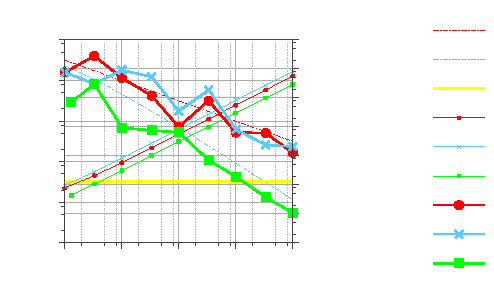
\includegraphics{converge}}%
    \gplfronttext
  \end{picture}%
\endgroup

	}
	\vspace{-2em}
	\caption{Convergence of maximum relative error $\Delta$ and run-time \(t\) according to the number of iterations $M$.}
	\label{fig:convergence}
	\vspace{-0.4cm}
\end{figure} 

Conceptually, we model the space of all \emph{valid} code words as an undirected, fully connected, weighted graph, where the code words are the vertices. Each valid code word is connected with every other valid one and the edge weights denote the \emph{Hamming distance} $d_H$ between the two code words. Thus, we only concentrate on the \emph{transitions} originating from valid code words to other valid ones, \emph{regardless of the coding}. Then, computing SDC probabilities requires two steps. First, we build a histogram over all transition weights, by which we get the numbers $c_b$ of undetectable $b$-bit flips:
\begin{Definition}
For a given code, $c_b$ denotes the number of transitions of weight \(b\) between valid code words.
\end{Definition}
The set \(\left\{c_b | b \in \left\{1,\dots,k\right\}\right\}\) is called \emph{weight distribution}. For AN coding, $c^A_b$ represents the count for a given \(A\). Second, we relate each $c_b$ to the respective total number of possible $b$-bit flips $\binom{n}{b}$.
Consequently, there can be $2^k \cdot \binom{n}{b}$ $b$-bit flips in all valid code words. This number includes all transitions from any \emph{valid} codeword to any other \emph{possible} code word. By that, when computing the weight distribution, we also have to count the transitions modeled in the graph twice (i.e., for each direction), because with a single error pattern we can make a transition in both direction. In total, this results in the SDC probability for $b$-bit flips, which we denote as:
\begin{equation}
p_b  = \frac{c_b}{2^k \cdot \binom{n}{b}}
\label{eq:sdc}
\end{equation}

Now, the challenge is to obtain \(c_b\) in an efficient manner. For non-linear codes like AN coding, \(c_b\) must be \emph{counted} in a brute force manner to the best of our knowledge. For AN coding, the convolution of the multiplication cannot be described in a way which allows simplifications. We use the following function to describe the naive approach:
\begin{equation}
	\delta_b (x, y) = \begin{cases}
		1,&\mathrm{if}\ {d_H(x,y)=b}, \\
		0,&\mathrm{if}\ {d_H(x,y)\neq b,}
	\end{cases}
	\qquad0\le b\le n\,.\nonumber
	\label{eq:delta}
\end{equation}
Then, we can compute the distance distribution as
\begin{equation}
	c_b = \sum_{\alpha\in\mathbb{C}} \sum_{\beta\in\mathbb{C}} \delta(\alpha, \beta)\,.
	\label{eq:naivecount}
\end{equation}
The complexity of Equation~(\ref{eq:naivecount}) is $\mathcal{O}(4^k)$, i.e. with each additional data bit, there are four times as many distances. In practice, it is half as much due to the symmetry (only one edge is computed and then counted twice). For parameter optimization, this might be run many thousands of times. Especially, for AN coding each odd \(A\) must be examined again for each data width \(|\mathbb{D}_\Theta|\) and with each additional bit, the number of candidates doubles. We call this naive approach \emph{exact}, as it examines all code words. For AN coding, Table~\ref{tab:runtimes} shows runtimes for the exact computation of the weight distribution for a single \(A\) using a single CPU, a single GPU, or a small cluster of 4 GPUs.




To mitigate the complexity, we use a sampling\=based approach, which approximates the weight distribution by comparing only a subset of all code words. Here, the main problem is the \emph{distribution} function for choosing the subset of code words. We investigated three different distributions: pseudo\=random (\(\sigma_\text{pseudo}\)), quasi\=random (\(\sigma_\text{quasi}\)), and grid-point (\(\sigma_\text{grid}\)). Note that \(\sigma_\text{pseudo}\) is prone to clustering, while \(\sigma_\text{quasi}\) fills the space more uniformly. The probabilistic error of Monte\=Carlo (pseudo\=random) is known to be $\mathcal{O}(\nicefrac{1}{\sqrt{M}})$ and for quasi\=Monte\=Carlo it is $\mathcal{O}(\nicefrac{(\log M)^q}{M})$ with number of dimensions $q$ and number of iterations $M$~\cite{montecarlo}. The grid\=point approach chooses regularly aligned samples, given by $\sigma_\text{grid}(r) = \nicefrac{(2^k\cdot r)}{M}$. If $M=2^k$, then the grid sampling yields the correct result, while random numbers still miss the solution due to collisions and gaps. Figure~\ref{fig:convergence} shows a comparison between the three distributions of convergence and runtime for the case \(k=24\) and \(A=61 \Rightarrow n=30\) and includes the theoretic Monte\=Carlo error boundaries. Pseudo- and quasi\=random numbers were generated with the cuRAND library. The 1D grid approximation outperforms the random distributions in virtually all cases, yielding smaller error \(\Delta\) and lower runtime \(t\). It is, furthermore, directly influenced by the value of \(M\), and we found that \emph{odd} values lead to much smaller errors than even ones.

\begin{algorithm}[t]
\caption{AN code distance distribution -- basic algorithm}
\label{alg:ancoding}
\begin{algorithmic}[1]
\Require $k\ge2$
\Require Value $A>0$, $n=k+h$, $h=\lceil\log_2(A)\rceil$
\Require Initial distance distribution $c^A_b=0,\,b=0,\ldots,n$
\Ensure Distance distribution $c^A$ of code $C_A$
\For{$\alpha=0,\ldots,(2^k-1)$} \Comment{outer loop is parallelized on GPU[s]} \label{alg:ancoding:1}
\For{$\beta=\sigma_\text{grid}(r),~r=0,\dots,M$}  \Comment{inner loop is processed by each thread} \label{alg:ancoding:2}
 \State $b \gets d_H( A\alpha, A\beta )$
 \State $c^A_b \gets c^A_b + 1$  \label{alg:ancoding:4}
\EndFor
\EndFor
\State \Return $c^A$
\end{algorithmic}
\end{algorithm}

Algorithm~\ref{alg:ancoding} shows the 1D grid approach for enumerating the weight distribution of an AN code. For GPU clusters, we distribute the outer loop evenly across the GPUs. When symmetry is exploited in line~\ref{alg:ancoding:2}, the workload size of each GPU is computed by:
\begin{equation}
	\lceil 2^k\omega_{i+1} \rceil - \lceil 2^k\omega_{i} \rceil,~w_i=1-\sqrt{1-\nicefrac{i}{N}},~0\le i<N \mbox{=\#GPUs}
	\label{eq:workload}
\end{equation}
$\omega_i$ is the solution of $\int_{i}^{i+1}1{-}x\,\mathrm{d}x=\nicefrac{1}{N}$ for equal work size areas. The maximal relative error of the estimation $\hat{c}^A_b$ is given by $\Delta = \max_{b>0} \frac{\mid c^A_b - \hat{c}^A_b \mid}{c^A_b}$ ($b=0$ is omitted due to $c^A_0=2^k$).

Algorithm~\ref{alg:ancoding} can be parallelized on GPUs, since the Hamming distances of two code
 words can be computed independently. We use CUDA C/C++ for programming Nvidia GPUs. As registers of GPUs are 32\=bit wide, the multi\=GPU implementation uses 32\=bit integers as long as the array elements in a thread do not overflow. From Equation~\ref{eq:sdc} follows $\max_b c_b^A\le\max_b 2^k\binom{n}{b}=2^k\binom{n}{n/2}$ and the upper bound for using 32\=bit integers is:
\[
c^A_{b,\mathrm{thread}}\le\frac{2^k\binom{n}{n/2}}{\mathrm{threads}}<2^{32}~.
\]
%It should be possible to use $\frac{2^k\binom{k}{k/2}}{\mathrm{threads}}$ as a lower bound, since higher values of $A$ make the distance distribution wider and flatter to keep the total sum equal to $4^k$. If \num4 GPUs are used with \num{64000} threads each, the 64\=bit implementation is used when $k\ge27$.
The GPU uses 64 bits for the global array, so the highest data bit width for the GPU algorithm is $k=33$. The range for each GPU is between $\lceil 2^k\omega_{i} \rceil$ and $\lceil 2^k\omega_{i+1} \rceil$ from Equation~\ref{eq:workload}. We use thread\=local arrays and one global array to avoid memory contention. Since local array indexing is dynamic and non\=uniform, it cannot be stored into the fast registers, as they are not addressable at run\=time. Hence, the local array is stored in local memory, which is L1 cached thread\=private global memory. To get scalable and flexible kernels, the outer loop strides by the size of a CUDA grid (threads per block $\times$ blocks per grid). The kernel is called with \lstinline{blocks}=$32\cdot\mathrm{numberOfMultiprocessors}$ and $128$ threads per block. After the local histogram is filled, atomic operations are used to add the values to the global distance distribution. The respective runtimes are shown in Table~\ref{tab:runtimes} on the right half. More details can be found in~\cite{kolditz2018}.



%Finally, we list all smallest super \(A\)s per bit flip weight which we computed until now in Table~\ref{tab:optimalAsComplete} and more super \(A\)s will be calculated. All up-to-date information will be available on our github project web page. 
%Note that super \(A\)s are not always increasing with larger \(|\mathbb{D}|\).

\begin{table}%
	\footnotesize
	\setlength{\tabcolsep}{0.7em} % for the horizontal padding
	\begin{tabular}{r|rrrrrrr}
		\toprule
		\multirow{2}{*}{\(|\mathbb{D}_\Theta|\)} & \multicolumn{6}{c}{minimal detectable bit flip weight} \\
		   & \multicolumn{1}{c}{1} & \multicolumn{1}{c}{2} & \multicolumn{1}{c}{3} & \multicolumn{1}{c}{4} & \multicolumn{1}{c}{5} & \multicolumn{1}{c}{6} & \multicolumn{1}{c}{7} \\
		\midrule
		 1 & \textbf{3}/2 &  \textbf{7}/3 &            15/4 &    \textbf{31}/5 &              63/6 &   \textbf{127}/7 &    255/8  \\
		 2 & \textbf{3}/2 & \textbf{13}/4 &   \textbf{53}/6 &            213/8 &   \textbf{853}/10 &          3285/12 & 13141/14  \\
		 3 & \textbf{3}/2 & \textbf{29}/5 &            45/6 &   \textbf{467}/9 &           1837/11 & \textbf{7349}/13 & 23733/15 \\
		 4 & \textbf{3}/2 &          27/5 &   \textbf{89}/7 &           933/10 &           6777/13 &         31385/15 \\
		 5 & \textbf{3}/2 & \textbf{29}/5 &           117/7 &           933/10 &           7085/13 &         31373/15 \\
		 6 & \textbf{3}/2 & \textbf{29}/5 &  \textbf{233}/8 &          1899/11 &           7837/13 &         62739/16 \\
		 7 & \textbf{3}/2 & \textbf{29}/5 &           217/8 &          1803/11 & \textbf{13963}/14 &         55831/16 \\
		 8 & \textbf{3}/2 & \textbf{29}/5 &  \textbf{233}/8 &          1939/11 & \textbf{13963}/14 &         55831/16 \\
		 9 & \textbf{3}/2 & \textbf{29}/5 &           185/8 &          1939/11 &          15717/14 &         55831/16 \\
		10 & \textbf{3}/2 & \textbf{61}/6 &           185/8 & \textbf{3739}/12 &          27425/15 \\
		11 & \textbf{3}/2 & \textbf{61}/6 &           451/9 & \textbf{3739}/12 &          27425/15 \\
		12 & \textbf{3}/2 & \textbf{61}/6 &  \textbf{463}/9 &          3737/12 &          29925/15 \\
		13 & \textbf{3}/2 & \textbf{61}/6 &  \textbf{463}/9 &          3349/12 &          27825/15 \\
		14 & \textbf{3}/2 & \textbf{61}/6 &  \textbf{463}/9 &          6717/13 &          63877/16 \\
		15 & \textbf{3}/2 & \textbf{61}/6 &  \textbf{463}/9 &          7785/13 &          63877/16 \\
		16 & \textbf{3}/2 & \textbf{61}/6 &  \textbf{463}/9 &          7785/13 &          63877/16 \\
		17 & \textbf{3}/2 & \textbf{61}/6 &           393/9 &          7785/13 &          63859/16 \\
		18 & \textbf{3}/2 & \textbf{61}/6 & \textbf{947}/10 &          7785/13 &          63859/16 \\
		... & ... \\
		28 & \textbf{3}/2 &         111/7 &          951/10 &         29685/15 \\
		29 & \textbf{3}/2 &         111/7 &          835/10 &        *29685/15 \\
		30 & \textbf{3}/2 &         125/7 &          835/10 &        *31693/15 \\
		31 & \textbf{3}/2 &         125/7 & \textbf{881}/10 &        *32211/15 \\
		32 & \textbf{3}/2 &         125/7 & \textbf{881}/10 &        *32417/15 \\
		\bottomrule
	\end{tabular}
	\caption{Smallest super \(A\)s per minimal detectable bit flip weight in the form \(A/|A|\). \textbf{Bold} numbers are prime. * obtained through grid approximation.}
	\label{tab:optimalAsComplete}
	\vspace{-3em}
\end{table}

\section{Github}
\label{sec:GitHub}
Finally, we would like to point out our project \emph{BRICS-DB} on GitHub\footnote{https://brics-db.github.io/} where our prototypical \emph{AHEAD} implementation is available, as well as our GPU implementation for computing distance distributions (SDC probability). We also provide the full table for all smallest super \(A\)s per bit flip weight which we computed until now. More super \(A\)s will be calculated and all updated information will be provided on github. Table~\ref{tab:optimalAsComplete} shows an excerpt of the current table of super \(A\)s.

%Actually, we computed all super \(A\)s for all \(1\leq|A|\leq16\) until time of submission.
